\begin{figure}
    \centering
    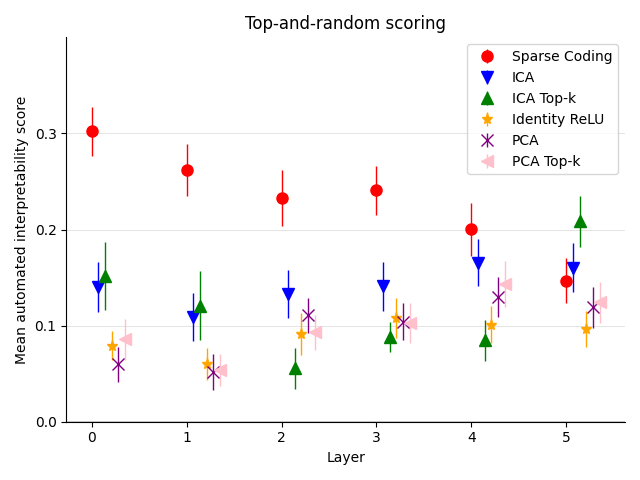
\includegraphics[width=.7\textwidth]{images/residual_top_random_topk_means_and_cis_new.png}
    \caption{Autointerpretation scores across layers for the residual stream, including top-K baselines for ICA and PCA.}
    \label{fig:topk}
\end{figure}

As mentioned in Section \ref{section:autointerp}, the comparison directions learnt by sparse coding and those in the baselines are not perfectly even. This is because, for example, a PCA direction is active to an entire half-space on one side of a hyperplane through the origin, whereas  a sparse coding feature activates on less than a full direction, being only on the far side of a hyperplane that does not intersect the origin. This is due to the bias applied before the activation, which is, in practice, always negative. To test whether this difference is responsible for the higher scores, we run a variant of PCA and ICA in which we have a fixed number of directions, K,  which can be active for any single datapoint. We set this K to be equal to the average number of active features for a sparse coding dictionary with ratio $R=1$ and $\alpha=8.6e-4$ trained on the layer in question. We compare the results in Figure \ref{fig:topk}, showing that this change does not explain more than a small fraction of the improvement in scores.  